\documentclass[11pt,a4paper]{article}

\usepackage[T1]{fontenc}
\usepackage[utf8]{inputenc}
\usepackage{lmodern}
\usepackage{geometry}
\usepackage{microtype}
\usepackage{amsmath,amssymb,mathtools,bm}
\usepackage{../Style/studentship-math-conventions}
\usepackage{booktabs,longtable,array,tabularx}
\usepackage{enumitem}
\usepackage{xcolor}
\usepackage{hyperref}
\usepackage{cleveref}
\usepackage{fancyhdr}
\usepackage{titlesec}
\usepackage{tikz}
\usetikzlibrary{positioning}
\usepackage{caption}
\usepackage{float}
\usepackage{siunitx}

\geometry{left=24mm,right=24mm,top=25mm,bottom=26mm}
\hypersetup{
  colorlinks=true,
  linkcolor=blue!45!black,
  citecolor=blue!45!black,
  urlcolor=blue!55!black,
  pdftitle={Consolidated Mathematical Model Specification for Hybrid Tohoku Tsunami and Barrier Analysis},
  pdfauthor={Summer Studentship Project},
  pdfsubject={2D NLSWE - 3D URANS-VOF hybrid tsunami model}
}
\setlength{\parindent}{0pt}
\setlength{\parskip}{0.58em}
\setlist{itemsep=0.25em,topsep=0.35em}
\renewcommand{\arraystretch}{1.18}
\pagestyle{fancy}
\setlength{\headheight}{14pt}
\fancyhf{}
\lhead{Summer Studentship}
\rhead{Consolidated Mathematical Model v1.0}
\cfoot{\thepage}
\setcounter{tocdepth}{2}
\setcounter{secnumdepth}{3}

\definecolor{Selected}{HTML}{E8F3EC}
\definecolor{Deferred}{HTML}{FFF3D9}
\definecolor{Unresolved}{HTML}{FCE8E6}
\definecolor{ProjectBlue}{HTML}{244A73}

\newcommand{\vect}[1]{\bm{#1}}
\newcommand{\dd}{\mathrm{d}}
\newcommand{\grad}{\nabla}
\newcommand{\Div}{\nabla\!\cdot}
\newcommand{\statusbox}[2]{%
  \begin{center}
  \fcolorbox{#1!70!black}{#1}{\parbox{0.92\linewidth}{\textbf{#2}}}
  \end{center}}
\newcommand{\selected}[1]{\statusbox{Selected}{Selected baseline: #1}}
\newcommand{\deferred}[1]{\statusbox{Deferred}{Deferred or stretch scope: #1}}
\newcommand{\unresolved}[1]{\statusbox{Unresolved}{Data-dependent or unresolved parameter: #1}}

\titleformat{\section}{\Large\bfseries\color{ProjectBlue}}{\thesection}{0.7em}{}
\titleformat{\subsection}{\large\bfseries\color{ProjectBlue!85!black}}{\thesubsection}{0.7em}{}
\titleformat{\subsubsection}{\normalsize\bfseries}{\thesubsubsection}{0.7em}{}

\begin{document}

\begin{titlepage}
\centering
\vspace*{18mm}
{\Huge\bfseries Consolidated Mathematical Model Specification\par}
\vspace{4mm}
{\LARGE Hybrid Regional--Local Simulation of the 2011 Tohoku Tsunami and Tsunami-Defence Interaction\par}
\vspace{10mm}
{\Large 2D Nonlinear Shallow-Water Equations\par}
{\Large $\longrightarrow$ One-Way Replay Coupling $\longrightarrow$ 3D URANS--VOF\par}
\vspace{15mm}
\begin{tabular}{rl}
\textbf{Project:} & Summer Studentship - tsunami-energy-dissipating barrier modelling\\
\textbf{Document status:} & Consolidated selected-model baseline\\
\textbf{Version:} & 1.0\\
\textbf{Date:} & 25 July 2026\\
\textbf{Primary study event:} & 11 March 2011 Tohoku earthquake and tsunami\\
\textbf{Regional trajectories:} & Epicentre--Kamaishi and epicentre--Sendai coastal plain\\
\end{tabular}
\vfill
\fcolorbox{ProjectBlue}{Selected}{\parbox{0.86\linewidth}{
\textbf{Purpose.} This document is the single mathematical and numerical specification for the active studentship baseline. It consolidates the modelling decisions confirmed through the Research workstream and identifies, without silently filling, the remaining data-dependent parameters. It is intended to govern subsequent software implementation and review.
}}
\vfill
\end{titlepage}

\pagenumbering{roman}
\begin{abstract}
The active studentship model is a hybrid regional--local tsunami simulation framework. A two-dimensional, depth-averaged, finite-volume nonlinear shallow-water model propagates the 2011 Tohoku tsunami across an evidence-defined corridor. Its nearshore solution is transferred through a one-way replay interface to a local three-dimensional, incompressible, immiscible two-phase Reynolds-averaged Navier--Stokes model with volume-of-fluid free-surface capture. The local model resolves interaction with fixed rigid tsunami-defence geometries and produces hydrodynamic pressure, shear, force, moment, impulse, overtopping, run-up, transmission and energy diagnostics. The operational turbulence baseline is URANS with the $k$--$\omega$ SST closure; LES, deformable structures, scour, damage and machine-learning-based optimisation remain deferred. The regional numerical baseline is a cell-centred finite-volume method on unstructured triangular cells with a Rusanov flux, hydrostatic reconstruction, positivity-preserving wetting--drying treatment, explicit CFL-controlled time integration and open/relaxation boundaries. The local numerical baseline is a collocated finite-volume URANS--VOF algorithm with bounded compressive phase transport, Rhie--Chow face-flux interpolation and PISO-like pressure correction. This specification records all confirmed choices, required invariants and verification stages, while flagging exact corridor extents, final source datasets, sponge widths, coupling reconstruction details and mesh-resolution values as case-definition parameters that remain to be locked from data.
\end{abstract}

\tableofcontents
\newpage

\section*{Document control and interpretation}
\addcontentsline{toc}{section}{Document control and interpretation}

This is a model specification, not a claim that verification, Tohoku validation or final production simulations have already been executed. Three statuses are used throughout:

\begin{itemize}
  \item \textbf{Selected baseline}: confirmed and implementation-authoritative unless later evidence forces a controlled revision.
  \item \textbf{Deferred}: deliberately outside the active baseline, but retained as an extension path.
  \item \textbf{Unresolved}: a value or detailed method that depends on datasets, calibration or benchmark evidence not yet finalised.
\end{itemize}

The Research workstream owns physical, mathematical, numerical, geometric and verification decisions. Software implements these decisions but must not redefine them implicitly. OpenFOAM is used as a mature architectural and numerical reference where it aligns with the selected model; it is not copied wholesale and does not override project research decisions \cite{projectHandoff,openfoamReview}.

\newpage
\pagenumbering{arabic}

\section{Project objective, scope and model hierarchy}

\subsection{Active objective}

The active objective is to recreate and analyse the hydrodynamic behaviour of the 2011 Tohoku tsunami in two representative east-coast trajectories, then quantify the performance of fixed rigid tsunami-defence classes under local three-dimensional impact. The present baseline prioritises:

\begin{itemize}
  \item physically traceable regional propagation;
  \item nearshore reconstruction and local replay;
  \item local free-surface and turbulent impact dynamics;
  \item wall-type versus obstacle/dissipating barrier comparisons;
  \item reproducible loading and transmission metrics;
  \item a software framework suitable for later optimisation and machine learning.
\end{itemize}

\selected{Impact modelling, Tohoku/local case comparison and barrier-class comparison are the active scientific scope.}

\deferred{Generative geometry, surrogate modelling, full optimisation, structural damage, deformable barriers, scour, two-way regional--local feedback and production LES are not part of the present baseline.}

\subsection{Hybrid model decomposition}

The governing hierarchy is
\begin{equation}
  \begin{aligned}
  \text{earthquake/source data}
  &\longrightarrow \text{regional 2D NLSWE}
  \longrightarrow \text{one-way replay interface}\\
  &\longrightarrow \text{local 3D URANS--VOF}
  \longrightarrow \text{barrier metrics}.
  \end{aligned}
\end{equation}

The decomposition is physical and computational:

\begin{enumerate}
  \item The regional model resolves propagation over a domain too large for a practical fully three-dimensional calculation.
  \item The local model is restricted to the defence and inundation region where vertical structure, wave breaking, air--water interface deformation, separation and obstacle loading matter.
  \item Coupling is one-way because the active goal is to replay regional forcing at a local boundary, not to return local reflections to the regional field.
\end{enumerate}

\begin{figure}[H]
\centering
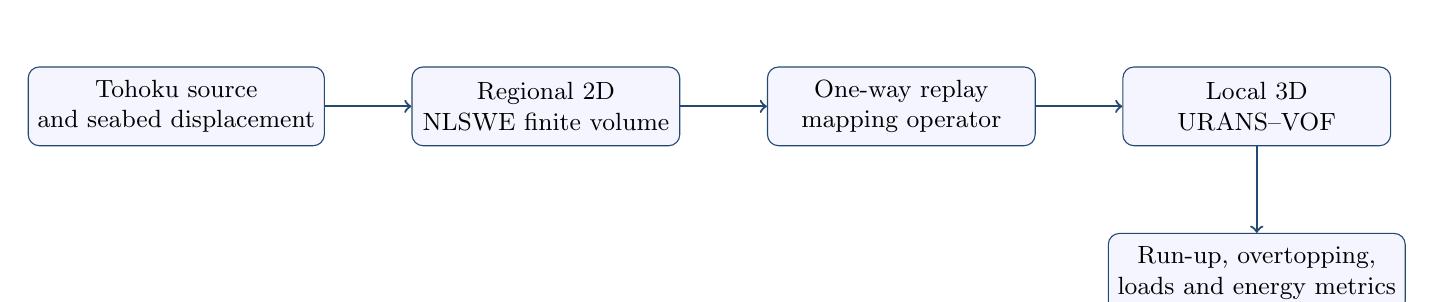
\begin{tikzpicture}[node distance=11mm, every node/.style={font=\small}, box/.style={draw=ProjectBlue, rounded corners, fill=blue!4, minimum width=34mm, minimum height=10mm, align=center}, arr/.style={->,thick,ProjectBlue}]
\node[box] (src) {Tohoku source\\and seabed displacement};
\node[box, right=of src] (r2d) {Regional 2D\\NLSWE finite volume};
\node[box, right=of r2d] (cpl) {One-way replay\\mapping operator};
\node[box, right=of cpl] (l3d) {Local 3D\\URANS--VOF};
\node[box, below=of l3d] (met) {Run-up, overtopping,\\loads and energy metrics};
\draw[arr] (src) -- (r2d);
\draw[arr] (r2d) -- (cpl);
\draw[arr] (cpl) -- (l3d);
\draw[arr] (l3d) -- (met);
\end{tikzpicture}
\caption{Selected hybrid modelling architecture.}
\end{figure}

\section{Coordinate system and evidence-defined corridor model}

\subsection{Geographic and local coordinates}

Let the earthquake epicentre be
\begin{equation}
  P_e=(\lambda_e,\phi_e)
\end{equation}
in geographic longitude--latitude coordinates. Let the selected coastal target be
\begin{equation}
  P_t=(\lambda_t,\phi_t).
\end{equation}
The two baseline targets are the Kamaishi region and the Sendai coastal plain. Geographic coordinates are first transformed into a metric projected coordinate system. A local orthonormal basis is then defined:
\begin{equation}
  \vect e_{x'}=\frac{\vect x_t-\vect x_e}{\|\vect x_t-\vect x_e\|},
  \qquad
  \vect e_{y'}=\begin{bmatrix}-e_{x',2}\\ e_{x',1}\end{bmatrix}.
\end{equation}
For a projected point $\vect x$, local coordinates are
\begin{equation}
  x'=(\vect x-\vect x_e)\cdot\vect e_{x'},
  \qquad
  y'=(\vect x-\vect x_e)\cdot\vect e_{y'}.
\end{equation}
The physical vertical coordinate is $z$, obtained from bathymetry/topography after consistent horizontal and vertical datum treatment.

\subsection{Corridor geometry}

The baseline corridor is a constant-width rectangle in the rotated frame:
\begin{equation}
\Omega_C=
\left\{(x',y'):
-L_{\mathrm{pre}}\le x'\le L_{\mathrm{target}}+L_{\mathrm{inland}},\quad
-\frac{W}{2}\le y'\le \frac{W}{2}
\right\}.
\end{equation}
Here:
\begin{itemize}
  \item $L_{\mathrm{pre}}$ is the source-side relief length before the epicentre;
  \item $L_{\mathrm{target}}$ is the epicentre-to-target distance;
  \item $L_{\mathrm{inland}}$ is the inland extent required to contain observed or modelled inundation and the barrier impact region;
  \item $W$ is the corridor width;
  \item $L_{\mathrm{sp}}$ is the width of each numerical relaxation/sponge region.
\end{itemize}

The initial proxy bearings retained by the Research handoff are approximately $338.9^\circ$ for Kamaishi and $262.6^\circ$ for Sendai, but these are not authoritative simulation parameters until final GIS target points are selected \cite{projectHandoff}.

\unresolved{Final $\theta$, $L_{\mathrm{pre}}$, $L_{\mathrm{inland}}$, $W$ and $L_{\mathrm{sp}}$ must be recomputed from the selected finite-fault footprint, observations, target geometry, coastline and mesh-resolution requirements.}

\subsection{Corridor construction rules}

The reproducible procedure is:
\begin{enumerate}
  \item define epicentre and target points in WGS84;
  \item transform to a metric CRS, preferably UTM Zone 54N or a local azimuthal-equidistant projection;
  \item construct the centreline and rotated basis;
  \item extend the centreline by $L_{\mathrm{pre}}$ and $L_{\mathrm{inland}}$;
  \item buffer by $W/2$ using flat end caps;
  \item clip bathymetry, topography, observations and defence geometry;
  \item harmonise datums and regrid onto the selected finite-volume mesh;
  \item record all transformations and source metadata in a data manifest.
\end{enumerate}

A narrowing corridor is not used merely to save cells. It is permitted only when the physical bay/coast geometry itself narrows and the computational boundary remains sufficiently remote from the dominant dynamics.

\section{Regional two-dimensional physical model}

\subsection{Assumptions}

The regional system is the depth-averaged nonlinear shallow-water model. Its use assumes:
\begin{itemize}
  \item horizontal length scales are much larger than water depth;
  \item vertical acceleration is secondary over the propagation region;
  \item pressure is hydrostatic in the depth-integrated model;
  \item the free surface is single-valued;
  \item wave dispersion is neglected in the operational baseline;
  \item density is constant and the water column is vertically integrated;
  \item bathymetry/topography are fixed after source initialisation;
  \item wetting and drying are required near shore and inland.
\end{itemize}

This approximation is appropriate for large-domain tsunami propagation and inundation, while the local three-dimensional model is introduced where the shallow-water assumptions cease to provide the required loading detail.

\subsection{State variables}

Let $b(x,y)$ denote bed elevation relative to the chosen vertical datum, positive upward. The water depth is $h\ge0$ and the free-surface elevation is
\begin{equation}
  \eta=h+b.
\end{equation}
Depth-averaged horizontal velocity is
\begin{equation}
  \vect u=(u,v)^T,
\end{equation}
and depth-integrated discharge is
\begin{equation}
  \vect q=h\vect u=(q_x,q_y)^T.
\end{equation}
The conservative state vector is
\begin{equation}
  \vect U=
  \begin{bmatrix}
  h\\ q_x\\ q_y
  \end{bmatrix}.
\end{equation}

\subsection{Conservative equations}

The selected regional equations are
\begin{equation}
  \frac{\partial \vect U}{\partial t}
  +\frac{\partial \vect F(\vect U)}{\partial x}
  +\frac{\partial \vect G(\vect U)}{\partial y}
  =\vect S_b+\vect S_f+\vect S_c+\vect S_e+\vect S_r,
  \label{eq:nlswe}
\end{equation}
with Cartesian fluxes
\begin{equation}
\vect F(\vect U)=
\begin{bmatrix}
q_x\\[1mm]
\dfrac{q_x^2}{h}+\dfrac{1}{2}gh^2\\[1mm]
\dfrac{q_xq_y}{h}
\end{bmatrix},
\qquad
\vect G(\vect U)=
\begin{bmatrix}
q_y\\[1mm]
\dfrac{q_xq_y}{h}\\[1mm]
\dfrac{q_y^2}{h}+\dfrac{1}{2}gh^2
\end{bmatrix}.
\end{equation}
The bathymetric source is
\begin{equation}
  \vect S_b=
  \begin{bmatrix}
  0\\ -gh\,\partial_x b\\ -gh\,\partial_y b
  \end{bmatrix}.
\end{equation}

\subsection{Bottom friction}

Manning friction is retained as the regional baseline. With Manning coefficient $n_M$,
\begin{equation}
  \vect S_f=
  \begin{bmatrix}
  0\\[1mm]
  -g n_M^2\dfrac{q_x\sqrt{q_x^2+q_y^2}}{h^{7/3}}\\[3mm]
  -g n_M^2\dfrac{q_y\sqrt{q_x^2+q_y^2}}{h^{7/3}}
  \end{bmatrix},
  \label{eq:manning}
\end{equation}
for wet cells. Numerical regularisation is required as $h\rightarrow0$ and must be consistent with the wetting--drying threshold.

\unresolved{Spatially varying Manning coefficients, roughness classes and urban/vegetation treatment are case-data inputs, not yet finalised constants.}

\subsection{Coriolis and optional forcing}

For sufficiently long propagation scales, the Coriolis source may be included:
\begin{equation}
  \vect S_c=
  \begin{bmatrix}
  0\\ f_c q_y\\ -f_c q_x
  \end{bmatrix},
  \qquad f_c=2\Omega_E\sin\phi.
\end{equation}
Wind and atmospheric-pressure forcing are not part of the baseline Tohoku event recreation and remain sensitivity options. They must not be enabled without evidence that they materially affect the selected event window.

\subsection{Earthquake and seabed displacement}

The source term $\vect S_e$ represents either initial free-surface displacement or time-dependent seabed motion. The simplest selected baseline is a finite-fault-derived vertical seabed displacement $\Delta b_e(x,y)$ mapped to the initial free surface:
\begin{equation}
  \eta(x,y,0)=\eta_0(x,y)+\Delta b_e(x,y),
  \qquad \vect q(x,y,0)=\vect 0,
\end{equation}
subject to comparison against a time-dependent rupture/seabed formulation where source duration is non-negligible. USGS finite-fault products provide an authoritative source candidate for the 2011 event \cite{usgsSource}.

\unresolved{The final finite-fault model, rupture timing and seabed-displacement operator remain RES-DAT/RES-MOD decisions. Static transfer is the implementation baseline until a dynamic source is selected.}

\subsection{Regional initial and boundary conditions}

The boundary is partitioned into source-side, inland/outflow and lateral artificial boundaries. Open/radiation behaviour is required; artificial lateral boundaries must not be treated as rigid coastal walls. A generic relaxation layer is represented by
\begin{equation}
  \vect S_r=-\sigma(\vect x)\left(\vect U-\vect U_{\mathrm{ref}}\right),
  \label{eq:relaxation}
\end{equation}
where $\sigma=0$ in the physical interior and increases smoothly across the sponge region. A polynomial profile may be written
\begin{equation}
  \sigma(s)=\sigma_{\max}\left(\frac{s}{L_{\mathrm{sp}}}\right)^m,
  \qquad 0\le s\le L_{\mathrm{sp}},
\end{equation}
with exponent $m\ge2$ used to reduce impedance discontinuity.

\unresolved{The exact radiation condition, sponge profile, $\sigma_{\max}$, exponent $m$ and sponge width are to be selected through reflection tests on the final mesh.}

\section{Regional finite-volume formulation}

\subsection{Mesh and geometric representation}

The selected regional discretisation uses unstructured triangular control volumes. Let
\begin{equation}
  \Omega_R=\bigcup_{i=1}^{N_c}K_i,
  \qquad V_i=|K_i|.
\end{equation}
Each oriented face $f$ has owner cell $P$, optional neighbour cell $N$, centre $\vect x_f$, length $A_f$ and owner-oriented area vector
\begin{equation}
  \vect S_f=A_f\vect n_f.
\end{equation}
For an internal face, $\vect S_f$ points from owner to neighbour. A face flux is evaluated once and contributes with opposite signs to the two adjacent residuals. This owner--neighbour pattern directly aligns with the selected cell-centred finite-volume model and is one of the OpenFOAM concepts adopted for the project \cite{openfoamReview}.

The authoritative mesh data are point coordinates, face connectivity, owners, neighbours, cell--face addressing and boundary-patch identity. Cell centres, areas, face centres and area vectors are derived geometry and should be calculated and validated from the topology.

\subsection{Semi-discrete conservation law}

The cell average is
\begin{equation}
  \overline{\vect U}_i(t)=\frac{1}{V_i}\int_{K_i}\vect U(\vect x,t)\,\dd V.
\end{equation}
Integrating \cref{eq:nlswe} gives
\begin{equation}
  \frac{\dd \overline{\vect U}_i}{\dd t}
  =-\frac{1}{V_i}
  \sum_{f\in\partial K_i}
  \epsilon_{if}\widehat{\vect F}_{n,f} A_f
  +\overline{\vect S}_i,
  \label{eq:fvsemi}
\end{equation}
where $\epsilon_{if}=+1$ when $i$ is the owner and $-1$ when it is the neighbour.

The residual is therefore
\begin{equation}
  \vect R_i(\vect U)
  =-\sum_{f\in\partial K_i}\epsilon_{if}\widehat{\vect F}_{n,f}A_f
  +V_i\overline{\vect S}_i,
\end{equation}
and the update equation is
\begin{equation}
  V_i\frac{\dd \overline{\vect U}_i}{\dd t}=\vect R_i.
\end{equation}
This establishes the role of the residual: it is the net discrete rate of conserved-quantity accumulation in a control volume, not merely an error check.

\subsection{Reconstruction}

The G1 baseline should begin with piecewise-constant states for verification, then introduce limited linear reconstruction:
\begin{equation}
  \vect U_{f,L}=\vect U_P+\Psi_P\grad\vect U_P\cdot(\vect x_f-\vect x_P),
\end{equation}
\begin{equation}
  \vect U_{f,R}=\vect U_N+\Psi_N\grad\vect U_N\cdot(\vect x_f-\vect x_N),
\end{equation}
where $\Psi$ denotes a monotonicity/positivity limiter. The specific gradient and limiter are not yet locked; constant and linear manufactured-field exactness are required before using the reconstruction in the tsunami solver.

\subsection{Rusanov numerical flux}

For a unit normal $\vect n=(n_x,n_y)^T$, define normal velocity
\begin{equation}
  u_n=u n_x+v n_y.
\end{equation}
The physical normal flux is
\begin{equation}
  \vect F_n(\vect U)=
  \begin{bmatrix}
  h u_n\\
  h u u_n+\frac{1}{2}gh^2n_x\\
  h v u_n+\frac{1}{2}gh^2n_y
  \end{bmatrix}.
\end{equation}
The selected baseline numerical flux is local Lax--Friedrichs/Rusanov:
\begin{equation}
  \widehat{\vect F}_{n}
  =\frac{1}{2}\left[\vect F_n(\vect U_L)+\vect F_n(\vect U_R)\right]
  -\frac{1}{2}s_{\max}(\vect U_R-\vect U_L),
  \label{eq:rusanov}
\end{equation}
where
\begin{equation}
  s_{\max}=\max\left(
  |u_{n,L}|+\sqrt{gh_L},
  |u_{n,R}|+\sqrt{gh_R}
  \right).
\end{equation}
HLL/HLLC variants are controlled later extensions; the Rusanov flux is retained because it is robust and provides a transparent first conservation baseline.

\subsection{Hydrostatic reconstruction and well-balancing}

A lake-at-rest equilibrium satisfies
\begin{equation}
  \vect q=\vect 0,
  \qquad \eta=h+b=\text{constant}.
\end{equation}
Naive discretisation of bed slope and pressure flux does not necessarily preserve this state. The selected approach is hydrostatic reconstruction \cite{audusse2004}. At a face, define
\begin{equation}
  b_f^*=\max(b_L,b_R),
\end{equation}
\begin{equation}
  h_L^*=\max(0,\eta_L-b_f^*),
  \qquad
  h_R^*=\max(0,\eta_R-b_f^*).
\end{equation}
Reconstructed conservative states use $h_L^*$ and $h_R^*$ with velocity retained where wet. Consistent hydrostatic pressure corrections are then added to the cell residual so that the discrete flux and bed source cancel at lake-at-rest.

\subsection{Wetting and drying}

A cell is classified dry when
\begin{equation}
  h_i<h_{\mathrm{dry}},
\end{equation}
where $h_{\mathrm{dry}}>0$ is a numerical threshold. Requirements are:
\begin{itemize}
  \item non-negative reconstructed depths;
  \item no division by vanishing depth;
  \item zero or controlled momentum in dry cells;
  \item flux limiting so an update cannot remove more water than a cell contains;
  \item consistent shoreline motion and rewetting;
  \item compatibility with hydrostatic reconstruction.
\end{itemize}

\unresolved{The exact positivity limiter and $h_{\mathrm{dry}}$ are to be selected from canonical shoreline and run-up benchmarks.}

\subsection{Explicit time integration and CFL control}

The baseline is an explicit strong-stability-preserving Runge--Kutta method, initially first-order forward Euler for component tests and then SSPRK2 or SSPRK3 for production. A cellwise gravity-wave CFL estimate is
\begin{equation}
  \Delta t_i
  \le
  C_{\mathrm{CFL}}
  \frac{V_i}
  {\displaystyle\sum_{f\in\partial K_i}A_f\left(|u_{n,f}|+\sqrt{gh_f}\right)}.
\end{equation}
The global timestep is
\begin{equation}
  \Delta t=\min_i\Delta t_i,
\end{equation}
with additional restrictions where source terms or relaxation layers require them.

\subsection{Regional solve sequence}

For accepted state $\vect U^n$:
\begin{enumerate}
  \item evaluate or update source forcing and boundary reference states;
  \item determine wet/dry classification;
  \item compute gradients and limited reconstructions where enabled;
  \item apply hydrostatic reconstruction at each face;
  \item calculate boundary or neighbour states;
  \item evaluate each numerical face flux once;
  \item accumulate equal-and-opposite owner/neighbour contributions;
  \item discretise bathymetry, friction, Coriolis and relaxation sources;
  \item select a stable timestep;
  \item advance the explicit Runge--Kutta stages;
  \item enforce positivity and admissibility;
  \item calculate conservation and shoreline diagnostics;
  \item accept the step or reduce $\Delta t$ and retry.
\end{enumerate}

\section{One-way regional-to-local replay coupling}

\subsection{Handoff variables}

The regional model must export, along the selected local inlet section and through time,
\begin{equation}
  \mathcal H_R=
  \left\{h_R,\eta_R,q_{x,R},q_{y,R},b_R\right\}.
\end{equation}
The depth-averaged regional velocity is
\begin{equation}
  \vect u_R=\frac{\vect q_R}{h_R}
\end{equation}
for wet states.

\subsection{Coupling operator}

Define a one-way mapping operator
\begin{equation}
  \mathcal M_{2D\rightarrow3D}:
  \mathcal H_R(s,t)
  \mapsto
  \left\{
  \alpha_{\mathrm{in}}(\vect x,t),
  \vect u_{\mathrm{in}}(\vect x,t),
  p_{\mathrm{in}}(\vect x,t),
  k_{\mathrm{in}}(\vect x,t),
  \omega_{\mathrm{in}}(\vect x,t)
  \right\}.
\end{equation}
At minimum, the mapped inlet must preserve:
\begin{enumerate}
  \item free-surface elevation;
  \item water-column depth;
  \item section-integrated volume discharge;
  \item dominant horizontal momentum direction;
  \item consistent bed/topographic datum;
  \item chronological phase and arrival time.
\end{enumerate}

A discharge-preservation condition is
\begin{equation}
  \int_{\Gamma_{\mathrm{in},w}(t)}
  \vect u_{\mathrm{in}}\cdot\vect n\,\dd A
  =
  \int_{\Gamma_R}
  \vect q_R\cdot\vect n_R\,\dd s.
  \label{eq:couplingmass}
\end{equation}
The local water/air indicator is reconstructed from the regional free surface:
\begin{equation}
  \alpha_{\mathrm{in}}(\vect x,t)=
  \begin{cases}
  1, & z<\eta_R(s,t),\\
  0, & z>\eta_R(s,t),
  \end{cases}
\end{equation}
with a numerically resolved transition across local interface cells.

\unresolved{The vertical inlet-velocity profile, turbulence inlet quantities, treatment of supercritical/subcritical transitions, temporal interpolation order and reflection-control method remain to be finalised. A depth-uniform profile is the simplest shallow-water-consistent baseline but is not recorded here as a completed calibration decision.}

\subsection{Why coupling is one-way}

The local model may generate reflected waves, but returning them to the regional model is deferred. One-way replay is accepted because:
\begin{itemize}
  \item the primary output is local defence loading under a prescribed Tohoku-scale incoming event;
  \item it avoids simultaneous multi-rate coupling and mesh communication;
  \item regional simulations can be archived and replayed across many defence geometries;
  \item it supports reproducibility and later optimisation campaigns.
\end{itemize}
Two-way coupling becomes necessary only if local reflection materially changes the regional incident field or if the local boundary lies too close to a strongly reflective feature.

\section{Local three-dimensional physical model}

\subsection{Domain and phase indicator}

The local fluid domain is $\Omega_L\subset\mathbb R^3$, containing water and air. Define the water volume fraction
\begin{equation}
  \alpha(\vect x,t)\in[0,1],
\end{equation}
with $\alpha=1$ in water and $\alpha=0$ in air. The interface occupies cells with $0<\alpha<1$.

Mixture properties are
\begin{equation}
  \rho(\alpha)=\alpha\rho_w+(1-\alpha)\rho_a,
\end{equation}
\begin{equation}
  \mu(\alpha)=\alpha\mu_w+(1-\alpha)\mu_a.
\end{equation}

\subsection{Incompressibility and momentum}

The selected one-fluid incompressible two-phase URANS equations are
\begin{equation}
  \Div\vect u=0,
  \label{eq:localcontinuity}
\end{equation}
\begin{equation}
  \frac{\partial(\rho\vect u)}{\partial t}
  +\Div(\rho\vect u\otimes\vect u)
  =-\grad p
  +\Div\left[\mu_{\mathrm{eff}}
  \left(\grad\vect u+\grad\vect u^T\right)\right]
  +\rho\vect g
  +\vect f_\sigma,
  \label{eq:localmomentum}
\end{equation}
where
\begin{equation}
  \mu_{\mathrm{eff}}=\mu+\mu_t.
\end{equation}
The surface-tension term $\vect f_\sigma$ may be represented using a continuum-surface-force model. For the full-scale tsunami baseline, gravity and inertia dominate, but retaining a consistent interface-force term is useful for numerical completeness and smaller verification cases.

\subsection{Volume-of-fluid transport}

The physical phase advection equation is
\begin{equation}
  \frac{\partial\alpha}{\partial t}
  +\Div(\alpha\vect u)=0.
  \label{eq:vofphysical}
\end{equation}
The finite-volume implementation adds bounded interface compression:
\begin{equation}
  \frac{\partial\alpha}{\partial t}
  +\Div(\alpha\vect u)
  +\Div\left[\alpha(1-\alpha)\vect u_c\right]=0,
  \label{eq:vofcompressed}
\end{equation}
where $\vect u_c$ is directed normal to the interface and is limited so that compression does not violate $0\le\alpha\le1$. The conceptual basis is the VOF method of Hirt and Nichols \cite{hirtNichols1981}.

\subsection{URANS $k$--$\omega$ SST closure}

The selected turbulence baseline is Menter's shear-stress-transport $k$--$\omega$ model \cite{menter1994}. In generic transport form,
\begin{equation}
  \frac{\partial(\rho k)}{\partial t}
  +\Div(\rho\vect u k)
  =P_k-\beta^*\rho k\omega
  +\Div\left[(\mu+\sigma_k\mu_t)\grad k\right],
  \label{eq:keq}
\end{equation}
\begin{equation}
  \frac{\partial(\rho\omega)}{\partial t}
  +\Div(\rho\vect u\omega)
  =\alpha_\omega\frac{\omega}{k}P_k
  -\beta\rho\omega^2
  +\Div\left[(\mu+\sigma_\omega\mu_t)\grad\omega\right]
  +2(1-F_1)\rho\sigma_{\omega2}
  \frac{\grad k\cdot\grad\omega}{\omega}.
  \label{eq:omegaeq}
\end{equation}
The eddy viscosity is limited by the SST shear-stress relation,
\begin{equation}
  \mu_t=\rho\frac{a_1k}{\max(a_1\omega,SF_2)},
  \label{eq:mut}
\end{equation}
where $F_1$ and $F_2$ blend near-wall and free-stream coefficient sets, and $S$ denotes an appropriate strain-rate magnitude. Standard SST coefficients and blending functions are to be used unless project-specific calibration is justified.

The production term is bounded to prevent excessive turbulence production near stagnation/impact zones. Turbulence quantities must remain positive:
\begin{equation}
  k>0,\qquad\omega>0.
\end{equation}

\subsection{Boundary partition}

The local boundary is
\begin{equation}
\partial\Omega_L=
\Gamma_{\mathrm{in}}\cup
\Gamma_{\mathrm{out}}\cup
\Gamma_{\mathrm{side}}\cup
\Gamma_{\mathrm{top}}\cup
\Gamma_T\cup
\Gamma_B.
\end{equation}
The selected meanings are:

\begin{longtable}{p{0.19\linewidth}p{0.74\linewidth}}
\toprule
Boundary & Physical and numerical role\\
\midrule
$\Gamma_{\mathrm{in}}$ & Offshore/local inlet forced by the one-way regional replay operator.\\
$\Gamma_{\mathrm{out}}$ & Inland or downstream open/radiation outlet with absorption where required.\\
$\Gamma_{\mathrm{side}}$ & Artificial lateral cuts representing continuation of the ocean/coastal field; not rigid walls.\\
$\Gamma_{\mathrm{top}}$ & Open atmosphere with atmospheric reference pressure and appropriate phase/velocity treatment.\\
$\Gamma_T$ & Fixed terrain/topography, no penetration; wall-shear model according to selected roughness treatment.\\
$\Gamma_B$ & Fixed rigid barrier or obstacle; no penetration with pressure and viscous traction extraction.\\
\bottomrule
\end{longtable}

\subsection{High-Reynolds-number and wall treatment}

The operational local flow is assumed turbulent and high Reynolds number. The baseline therefore uses scalable wall functions rather than resolving every viscous sublayer. This choice limits near-wall shear fidelity and requires wall-normal mesh quality and $y^+$ monitoring. Low-Re fully resolved walls and LES are deferred comparison models rather than default production settings.

\section{Local finite-volume and pressure-correction formulation}

\subsection{Collocated cell-centred storage}

The local mesh is cell-centred and collocated. For cell $K_i$ the stored unknowns are
\begin{equation}
  \alpha_i,\ \vect u_i,\ p_i,\ k_i,\ \omega_i,\ \rho_i,\ \mu_i,\ \mu_{t,i}.
\end{equation}
For oriented face $f$,
\begin{equation}
  \phi_f=A_f(\vect u_f\cdot\vect n_f)
  =\vect u_f\cdot\vect S_f
\end{equation}
is the volumetric face flux.

The mesh/field structure adopts from OpenFOAM the separation of topology, geometry, dense fields and boundary patches, but rejects its full object-registry and macro-based runtime-selection systems \cite{openfoamReview}.

\subsection{Finite-volume momentum predictor}

After phase update and mixture-property evaluation, the discretised momentum equation is written
\begin{equation}
  a_P\vect u_P^*
  =\vect H_P- V_P\grad p^n_P+\vect b_P,
  \label{eq:mompredict}
\end{equation}
where $a_P$ contains implicit transient/diffusive and selected convective coefficients, $\vect H_P$ collects neighbour and explicit contributions, and $\vect b_P$ contains gravity and other body terms. The predicted velocity $\vect u^*$ does not generally satisfy discrete continuity.

\subsection{Rhie--Chow face interpolation}

Direct interpolation of collocated pressure and velocity can produce checkerboard pressure modes. The selected remedy is Rhie--Chow pressure-weighted face-flux interpolation \cite{rhieChow1983}. In schematic form,
\begin{equation}
  \phi_f^*=\phi_{H,f}
  -D_f\left[(\grad p)_f\cdot\vect S_f
  -\overline{\grad p}_f\cdot\vect S_f\right],
  \label{eq:rhie}
\end{equation}
where $D_f$ derives from inverse momentum coefficients and the bracket represents a pressure correction constructed to suppress decoupling without adding excessive dissipation.

\subsection{PISO-like pressure correction}

Write
\begin{equation}
  p^{n+1}=p^n+p',
  \qquad
  \vect u^{n+1}=\vect u^*+\vect u'.
\end{equation}
The velocity correction follows from the pressure correction:
\begin{equation}
  \vect u'_P=-d_P\grad p'_P.
\end{equation}
Substituting the corrected flux into discrete continuity yields a Poisson-like pressure-correction equation
\begin{equation}
  \sum_{f\in\partial K_P}D_f(\grad p')_f\cdot\vect S_f
  =\sum_{f\in\partial K_P}\phi_f^*.
  \label{eq:pcorr}
\end{equation}
Pressure, velocity and face flux are corrected repeatedly until the mass imbalance is below tolerance. The selected procedure is PISO-like and follows the operator-splitting/pressure-correction principles of Issa \cite{issa1986a,issa1986b}.

\subsection{Bounded phase transport}

The VOF update must satisfy:
\begin{equation}
  0\le\alpha_i^{n+1}\le1.
\end{equation}
Convective and compressive phase fluxes are limited consistently. After updating $\alpha$, mixture properties are recomputed before the momentum predictor. Interface Courant number is monitored separately from bulk flow CFL.

\subsection{Time-step restrictions}

The local timestep is selected from the minimum of relevant constraints:
\begin{equation}
  \Delta t=\theta_t\min\left(
  \Delta t_{\mathrm{conv}},
  \Delta t_{\alpha},
  \Delta t_g,
  \Delta t_\nu
  \right),
\end{equation}
where $0<\theta_t\le1$ is a safety factor. Representative estimates are
\begin{equation}
  \Delta t_{\mathrm{conv},i}
  \sim \frac{V_i}{\sum_f|\phi_f|},
\end{equation}
\begin{equation}
  \Delta t_{g,i}\sim\frac{\Delta \ell_i}{\sqrt{gH_i}},
  \qquad
  \Delta t_{\nu,i}\sim\frac{\Delta \ell_i^2}{\nu_{\mathrm{eff},i}}.
\end{equation}
The exact interface-CFL definition depends on the selected compressive VOF discretisation.

\subsection{Accepted local solve sequence}

Given accepted fields at time level $n$:
\begin{enumerate}[label=\arabic*.]
  \setcounter{enumi}{-1}
  \item interpolate regional forcing to the local inlet;
  \item select $\Delta t$ from convective, interface, gravity-wave and diffusion restrictions;
  \item update boundary-face states;
  \item solve the bounded compressive VOF equation for $\alpha$;
  \item update $\rho$ and $\mu$ from $\alpha$;
  \item assemble and solve the URANS momentum predictor for $\vect u^*$;
  \item construct Rhie--Chow pressure-consistent face fluxes $\phi^*$;
  \item solve the pressure-correction equation for $p'$;
  \item correct pressure, velocity and face fluxes;
  \item repeat pressure correctors until mass residual is acceptable;
  \item solve $k$ and $\omega$ using corrected velocity and flux;
  \item update $\mu_t$ and $\mu_{\mathrm{eff}}$;
  \item apply scalable wall-function quantities at terrain and barrier walls;
  \item extract free-surface, loading, run-up, overtopping, transmission and energy metrics;
  \item check all acceptance criteria;
  \item accept and advance, or reject the step and reduce $\Delta t$.
\end{enumerate}

\section{Barrier geometry classes and response quantities}

\subsection{Active geometry classes}

Two baseline classes are retained:
\begin{enumerate}
  \item \textbf{Wall-type}: continuous seawall, breakwater or rigid barrier producing reflection, overtopping and concentrated loading.
  \item \textbf{Obstacle/dissipating type}: arrays or discrete obstacles intended to redistribute momentum, promote separation/turbulence and reduce transmitted energy.
\end{enumerate}

The geometry model must record at minimum:
\begin{itemize}
  \item position and orientation relative to the incoming corridor axis;
  \item crest/elevation and total height;
  \item width, thickness and length;
  \item spacing and count for obstacle arrays;
  \item blockage ratio and porosity proxy where relevant;
  \item shape/orientation category;
  \item reference point for moment calculation;
  \item fixed rigid-surface identity and boundary patch.
\end{itemize}

\deferred{Automatic geometry generation, material compliance, failure, scour and fluid--structure interaction.}

\subsection{Hydrodynamic traction, force and moment}

The traction on barrier surface $\Gamma_B$ is
\begin{equation}
  \vect t_B=-p\vect n+\bm\tau\vect n,
\end{equation}
where
\begin{equation}
  \bm\tau=\mu_{\mathrm{eff}}\left(\grad\vect u+\grad\vect u^T\right)
\end{equation}
under the selected effective-viscosity model. The resultant force is
\begin{equation}
  \vect F_B(t)=\int_{\Gamma_B}\vect t_B\,\dd A,
\end{equation}
and the moment about reference point $\vect x_0$ is
\begin{equation}
  \vect M_B(t)=\int_{\Gamma_B}
  (\vect x-\vect x_0)\times\vect t_B\,\dd A.
\end{equation}
The force impulse is
\begin{equation}
  \vect I_B(t_1,t_2)=\int_{t_1}^{t_2}\vect F_B(t)\,\dd t.
\end{equation}
Pressure and viscous contributions must be separately available so later structural analyses can distinguish dominant loading mechanisms.

\subsection{Run-up and overtopping}

For terrain or barrier surface elevation $z_s(\vect x)$, local inundation depth is
\begin{equation}
  d(\vect x,t)=\max\left(0,\eta(\vect x,t)-z_s(\vect x)\right).
\end{equation}
Maximum run-up elevation is
\begin{equation}
  R_{\max}=\max_{\vect x\in\Gamma_T,t}\left[\eta(\vect x,t)-\eta_0\right]
\end{equation}
subject to the project convention for vertical datum and shoreline extraction.

For a crest section $\Gamma_c$, overtopping discharge is
\begin{equation}
  Q_{\mathrm{over}}(t)=
  \int_{\Gamma_c\cap\{\alpha>\alpha_w\}}
  \vect u\cdot\vect n_c\,\dd A,
\end{equation}
and cumulative overtopped volume is
\begin{equation}
  V_{\mathrm{over}}(t)=\int_0^tQ_{\mathrm{over}}(\tau)\,\dd\tau.
\end{equation}

\subsection{Transmission and energy metrics}

At incident and transmitted control sections, define water-phase volume flux
\begin{equation}
  Q(t)=\int_{\Gamma_w(t)}\vect u\cdot\vect n\,\dd A.
\end{equation}
A free-surface amplitude transmission coefficient may be defined by
\begin{equation}
  K_\eta=\frac{\eta_{\mathrm{trans,max}}}{\eta_{\mathrm{inc,max}}},
\end{equation}
and a momentum-flux transmission coefficient by
\begin{equation}
  K_M=
  \frac{\displaystyle\int_{t_1}^{t_2}\int_{\Gamma_{\mathrm{trans}}}
  \rho(\vect u\cdot\vect n)^2\,\dd A\,\dd t}
  {\displaystyle\int_{t_1}^{t_2}\int_{\Gamma_{\mathrm{inc}}}
  \rho(\vect u\cdot\vect n)^2\,\dd A\,\dd t}.
\end{equation}
A mechanical-energy flux diagnostic may use
\begin{equation}
  \mathcal P_E(t)=
  \int_{\Gamma_w(t)}
  \left(p+\frac{1}{2}\rho\|\vect u\|^2+\rho gz\right)
  (\vect u\cdot\vect n)\,\dd A.
\end{equation}
The energy-transmission coefficient is then
\begin{equation}
  K_E=
  \frac{\int_{t_1}^{t_2}\mathcal P_{E,\mathrm{trans}}\,\dd t}
  {\int_{t_1}^{t_2}\mathcal P_{E,\mathrm{inc}}\,\dd t}.
\end{equation}

\unresolved{The precise control-section positions, signal separation between incident/reflected components and the final energy definition require a dedicated metrics specification before comparative simulations.}

\section{Data model and case-study inputs}

\subsection{Selected source hierarchy}

The case requires bathymetry/topography, earthquake source data, deep-ocean/coastal observations, run-up/inundation observations and defence geometry. The current source hierarchy is:

\begin{longtable}{p{0.20\linewidth}p{0.25\linewidth}p{0.46\linewidth}}
\toprule
Data category & Primary candidate & Project role and limitation\\
\midrule
Japan bathymetry & JODC J-EGG500 & Regional/local topobathymetry around Japan; 500 m gridded bathymetric product assembled from survey data \cite{jegg500}. Finer local reconstruction may still be required.\\
Outer-domain bathymetry & GEBCO or NOAA ETOPO & Fallback/outer-domain coverage where J-EGG500 coverage or licensing is insufficient.\\
Onshore elevation & GSI DEM & Japan-specific terrestrial elevation; horizontal/vertical datum and resolution must be preserved in the manifest \cite{gsiDem}.\\
Earthquake source & USGS finite-fault products & Event geometry, slip and rupture candidates for source reconstruction \cite{usgsSource}.\\
Deep-ocean observations & NOAA/NCEI DART & Arrival-time and deep-water waveform comparison for 11 March 2011 \cite{noaaDart}.\\
Historical/run-up database & NOAA/NCEI Global Historical Tsunami Database & Event and run-up records, with source-quality screening \cite{noaaHistorical}.\\
Field run-up/inundation & Tohoku Joint Survey Group / Mori et al. & High-density Japanese coastal run-up and inundation evidence \cite{mori2011,mori2012}.\\
Defence geometry & Kamaishi breakwater and site-specific reports & Primary real-defence recreation candidate; exact as-built/pre-event geometry remains to be assembled.\\
\bottomrule
\end{longtable}

\subsection{Required provenance}

Every dataset must record:
\begin{itemize}
  \item provider and product version;
  \item access date and licence;
  \item spatial/temporal coverage;
  \item horizontal CRS and vertical datum;
  \item native resolution and resampling method;
  \item no-data handling;
  \item interpolation and smoothing operations;
  \item source uncertainty and known omissions;
  \item file hash and generated-artifact lineage.
\end{itemize}

\subsection{Authoritative versus derived data}

Source files and original metadata are immutable inputs. Corridor polygons, clipped rasters, interpolated mesh fields, reconstructed source displacement and local inlet time series are derived artefacts. The latter must be reproducible from the former through a versioned data-manifest workflow.

\section{OpenFOAM alignment and project-specific adaptation}

OpenFOAM is a reference because its mature finite-volume architecture separates reusable libraries, mesh topology, finite-volume geometry, dense fields, operators, solvers, I/O and visualisation. The project adopts only the parts that directly support the selected model \cite{openfoamReview}.

\begin{longtable}{p{0.27\linewidth}p{0.16\linewidth}p{0.49\linewidth}}
\toprule
OpenFOAM pattern & Decision & Project adaptation\\
\midrule
Library-first modularity & Adopt & Numerical libraries remain independent of Qt; CLI/GUI are thin applications.\\
Owner/neighbour face addressing & Adopt & Used for both regional and local conservative flux accumulation.\\
Topology/geometry separation & Adopt & Coordinates/connectivity are authoritative; centres, measures and area vectors are derived.\\
Dense field arrays & Adopt & Cell/face fields use contiguous memory and lightweight views.\\
Boundary patches & Adopt & Boundary identity is separated from interior traversal and later condition behaviour.\\
General polyhedral mesh & Adapt & First regional implementation is explicitly 2D triangular; local solver retains a 3D unstructured path.\\
$polyMesh$/$fvMesh$ class hierarchy & Adapt & Smaller project-specific topology and geometry interfaces; no global registry inheritance.\\
Runtime selection macros & Reject/defer & Direct construction or small typed factories until multiple genuine runtime alternatives exist.\\
Native directory-per-time output & Reject & HDF5/XDMF is the authoritative scientific-data path; export formats are adapters.\\
MPI processor boundaries & Defer & Data structures avoid blocking future partitioning, but serial correctness comes first.\\
Solver-integrated rendering & Reject & Visualisation consumes immutable or persisted outputs; numerical kernels do not depend on Qt.\\
\bottomrule
\end{longtable}

The rule is strict: project research decisions govern the mathematical model. OpenFOAM supplies proven implementation patterns only when they align with those decisions.

\section{Verification, validation and acceptance framework}

\subsection{Three-level credibility hierarchy}

The selected hierarchy is:
\begin{enumerate}
  \item \textbf{V1 - solver capability and verification}: unit, conservation, manufactured/analytical and canonical benchmark tests.
  \item \textbf{V2 - Tohoku hydrodynamic validation}: deep-ocean waveform, arrival time, coastal height, run-up and inundation comparison.
  \item \textbf{V3 - impact and loading validation}: free-surface impact, pressure, force, impulse and obstacle/barrier benchmarks.
\end{enumerate}
No final validation claim is made until all relevant levels have documented data, uncertainty and acceptance criteria.

\subsection{Regional verification requirements}

Minimum tests include:
\begin{itemize}
  \item constant-state preservation;
  \item lake-at-rest well-balancing over variable bathymetry;
  \item positivity and wet/dry-front propagation;
  \item conservation across an internal face;
  \item dam-break and bore propagation;
  \item solitary-wave run-up, including comparison with analytical/benchmark results such as Synolakis \cite{synolakis1987};
  \item mesh-refinement and observed-order studies;
  \item sponge-layer reflection measurement;
  \item coupling-section discharge conservation.
\end{itemize}

\subsection{Local verification requirements}

Minimum tests include:
\begin{itemize}
  \item divergence-free pressure-correction benchmark;
  \item collocated-grid pressure-decoupling test;
  \item bounded VOF advection and interface-shape tests;
  \item hydrostatic free-surface equilibrium;
  \item dam-break/free-surface impact benchmark;
  \item turbulence transport positivity;
  \item wall-function and $y^+$ monitoring;
  \item force and moment integration on a known body;
  \item mass conservation over accepted timesteps;
  \item timestep-rejection and restart consistency.
\end{itemize}

\subsection{Numerical-error reporting}

Grid and timestep studies should report:
\begin{equation}
  e_h=\|\phi_h-\phi_{\mathrm{ref}}\|,
\end{equation}
observed order
\begin{equation}
  p=\frac{\ln(e_{h_1}/e_{h_2})}{\ln(h_1/h_2)},
\end{equation}
and a grid-convergence indicator where applicable, following accepted verification practice \cite{roache1994}.

\subsection{Runtime acceptance checks}

A regional step is admissible only when:
\begin{itemize}
  \item $h\ge0$ within tolerance;
  \item CFL restrictions are satisfied;
  \item non-finite values are absent;
  \item conservation error is within the test-specific tolerance;
  \item wet/dry classification is internally consistent.
\end{itemize}

A local step is admissible only when:
\begin{itemize}
  \item $0\le\alpha\le1$ within tolerance;
  \item $k>0$ and $\omega>0$;
  \item continuity/mass residual is below tolerance;
  \item pressure, momentum and turbulence solver convergence criteria are met;
  \item bulk and interface CFL constraints are satisfied;
  \item required output state is synchronised and finite.
\end{itemize}

\section{Selected assumptions, limitations and unresolved decisions}

\subsection{Confirmed assumptions}

\begin{enumerate}
  \item Regional propagation is adequately represented by depth-averaged NLSWE for the active study.
  \item The local impact region requires a three-dimensional two-phase model.
  \item Regional-to-local coupling is one-way replay.
  \item Terrain and barriers are fixed and rigid.
  \item Air is retained numerically through VOF.
  \item URANS $k$--$\omega$ SST is the operational turbulence baseline.
  \item Regional discretisation is unstructured triangular cell-centred finite volume.
  \item Local discretisation is collocated cell-centred finite volume with PISO-like pressure correction and Rhie--Chow interpolation.
  \item Barrier comparison includes wall and obstacle/dissipating classes.
  \item Active solver fields reside in contiguous memory; HDF5 is persistence, not stencil memory.
\end{enumerate}

\subsection{Principal limitations}

\begin{itemize}
  \item Regional NLSWE neglect frequency dispersion and vertical flow structure.
  \item One-way coupling neglects feedback from local reflections.
  \item URANS models rather than resolves the full turbulent spectrum.
  \item Wall functions limit near-wall detail and depend on mesh quality.
  \item Rigid barriers exclude deformation, failure, porosity evolution and scour.
  \item Air compressibility and entrained sediment/debris are excluded.
  \item Corridor boundaries are artificial and require measured reflection control.
  \item Source and terrain accuracy are limited by available datasets and datum transformations.
\end{itemize}

\subsection{Unresolved parameter register}

\begin{longtable}{p{0.28\linewidth}p{0.61\linewidth}}
\toprule
Parameter/decision & Required resolution evidence\\
\midrule
Final Kamaishi and Sendai target coordinates & GIS selection using impact observations and defence geometry.\\
$L_{\mathrm{pre}}$, $L_{\mathrm{inland}}$, $W$ & Finite-fault footprint, run-up/inundation envelope, boundary-distance and mesh-cost study.\\
Sponge width/profile & Reflection benchmarks on the selected mesh and dominant wave spectrum.\\
Final bathymetry/topography blend & Product coverage, licence, datum, resolution and overlap-error analysis.\\
Finite-fault/source model & Comparison of USGS and other accepted source inversions against DART/coastal observations.\\
Regional friction map & Land-cover/roughness evidence and sensitivity analysis.\\
Wet/dry threshold and limiter & Canonical shoreline and run-up benchmarks.\\
Regional reconstruction/limiter & Manufactured fields, monotonicity and event-scale convergence.\\
2D-to-3D vertical velocity profile & Discharge preservation, inlet stability and local sensitivity tests.\\
Local inlet $k$ and $\omega$ & Turbulence-intensity/length-scale assumption and sensitivity.\\
VOF compression coefficient & Interface boundedness and advection benchmark.\\
PISO corrector count/tolerances & Mass residual and temporal-accuracy study.\\
Wall roughness and wall-function parameters & Material/site evidence and $y^+$ study.\\
Barrier energy/transmission control sections & Metrics specification and reflection separation method.\\
Mesh resolution/refinement zones & Grid-convergence, bathymetry curvature, free surface and loading gradients.\\
\bottomrule
\end{longtable}

\section{Implementation handoff requirements}

\subsection{Authority and sequencing}

Software implementation must follow this authority chain:
\begin{equation}
  \begin{aligned}
  \text{research model}
  &\rightarrow \text{mathematical contract}
  \rightarrow \text{numerical contract}\\
  &\rightarrow \text{software interface}
  \rightarrow \text{verified implementation}.
  \end{aligned}
\end{equation}
OpenFOAM-inspired code may accelerate implementation only when the mathematical role and ownership match the selected project model.

\subsection{First simulation implementation sequence}

The recommended sequence is:
\begin{enumerate}
  \item validated finite-volume topology and derived geometry;
  \item typed cell/face fields with mesh compatibility;
  \item interpolation and gradient primitives;
  \item boundary-patch framework;
  \item regional conservative state and admissibility;
  \item Rusanov flux and residual assembly;
  \item hydrostatic reconstruction and source balancing;
  \item wetting--drying and explicit timestep control;
  \item regional boundary/sponge treatment;
  \item coupling replay format and mapping tests;
  \item local URANS--VOF scaffold and pressure correction;
  \item barrier metric extraction;
  \item HDF5/XDMF persistence and GUI consumption.
\end{enumerate}

\subsection{Core software invariants derived from the model}

\begin{itemize}
  \item Mesh topology and fields are separate objects.
  \item Point coordinates/connectivity are authoritative; geometry is derived and validated.
  \item Every internal face has one owner and one neighbour; boundary faces have one owner and one patch.
  \item A face area vector is oriented owner-to-neighbour or outward from the owner.
  \item Internal numerical fluxes are evaluated once and accumulated with opposite signs.
  \item Field storage is contiguous and associated with one mesh identity and location.
  \item Operators receive references/views and do not repeatedly deep-copy whole fields.
  \item Numerical libraries contain no Qt types and no HDF5 handles.
  \item Output frames are immutable once published.
  \item Serial reference kernels remain available after any parallel backend is introduced.
\end{itemize}

\section{Consolidated decision table}

\begin{longtable}{p{0.26\linewidth}p{0.26\linewidth}p{0.40\linewidth}}
\toprule
Area & Selected choice & Rationale\\
\midrule
Regional physics & 2D depth-averaged NLSWE & Computationally appropriate for large-domain tsunami propagation and inundation.\\
Regional mesh & Unstructured triangles & Fits irregular corridor coastlines and supports local refinement.\\
Regional flux & Rusanov baseline & Robust, transparent and suitable for first verified conservation implementation.\\
Bathymetry balance & Hydrostatic reconstruction & Preserves lake-at-rest and supports wet/dry fronts \cite{audusse2004}.\\
Regional time integration & Explicit CFL-controlled SSPRK & Matches hyperbolic propagation and provides clear stability control.\\
Coupling & One-way regional-to-local replay & Reusable forcing, lower complexity and appropriate current scientific objective.\\
Local physics & Incompressible water--air URANS--VOF & Resolves three-dimensional free-surface impact and barrier loading.\\
Turbulence & $k$--$\omega$ SST URANS & Operational high-Re wall-bounded/separated-flow baseline.\\
Local mesh/storage & Collocated cell-centred finite volume & Shared conservative framework and practical unstructured-grid support.\\
Pressure--velocity coupling & PISO-like correction with Rhie--Chow & Transient incompressible coupling and collocated pressure stability.\\
Barrier representation & Fixed rigid wall and obstacle classes & Isolates hydrodynamic performance before structural extensions.\\
Persistence & HDF5/XDMF, not active solver memory & Structured large-array storage, restart and visualisation handoff.\\
Visualisation & Separate consumer of solver data & Prevents GUI dependencies from contaminating numerical libraries.\\
OpenFOAM use & Adopt/adapt selected patterns only & Saves implementation effort while preserving project-specific research authority.\\
\bottomrule
\end{longtable}

\section{Conclusion}

The selected model is a one-way hybrid 2D NLSWE--3D URANS--VOF framework for the 2011 Tohoku tsunami and fixed rigid barrier interaction. Its regional and local formulations, numerical identities, coupling contract, geometry classes, output metrics and verification hierarchy are now sufficiently defined to govern implementation. The remaining uncertainties are primarily case-data, resolution, boundary-calibration and coupling-reconstruction parameters. Those uncertainties must be resolved explicitly through the Research data and verification workstreams; they must not be hidden inside software defaults.

The immediate implementation consequence is that finite-volume topology, geometry and field data structures are not generic preliminary coding. They are direct representations of this mathematical model and must therefore be reviewed against the equations, conservation rules and selected OpenFOAM adaptations before further code is approved.

\appendix
\section{Notation}

\begin{longtable}{p{0.18\linewidth}p{0.72\linewidth}}
\toprule
Symbol & Meaning\\
\midrule
$h$ & Regional water depth.\\
$\eta$ & Free-surface elevation.\\
$b$ & Bed elevation, positive upward.\\
$\vect q=(q_x,q_y)$ & Depth-integrated discharge.\\
$\vect u$ & Velocity; depth-averaged in the regional model, 3D in the local model.\\
$\vect U$ & Regional conservative state $[h,q_x,q_y]^T$.\\
$K_i,V_i$ & Control volume and its area/volume.\\
$A_f,\vect n_f,\vect S_f$ & Face measure, unit normal and oriented area vector.\\
$\alpha$ & Water volume fraction.\\
$\rho,\mu,\mu_t$ & Mixture density, molecular dynamic viscosity and turbulent dynamic viscosity.\\
$p$ & Local pressure variable.\\
$k,\omega$ & Turbulent kinetic energy and specific dissipation rate.\\
$\phi_f$ & Local volumetric face flux.\\
$\Gamma_B$ & Barrier surface.\\
$L_{\mathrm{pre}}$ & Source-side corridor relief length.\\
$L_{\mathrm{inland}}$ & Inland corridor extent.\\
$W$ & Corridor width.\\
$L_{\mathrm{sp}}$ & Sponge/relaxation-layer width.\\
\bottomrule
\end{longtable}

\section{Reference two-triangle finite-volume fixture}

For the first topology and operator tests, use vertices
\begin{equation}
  \vect x_0=(0,0),\quad
  \vect x_1=(1,0),\quad
  \vect x_2=(1,1),\quad
  \vect x_3=(0,1),
\end{equation}
with triangles
\begin{equation}
  K_0=(0,1,2),\qquad K_1=(0,2,3).
\end{equation}
Then
\begin{equation}
  V_0=V_1=\frac{1}{2},
  \qquad
  \vect x_{K_0}=\left(\frac{2}{3},\frac{1}{3}\right),
  \qquad
  \vect x_{K_1}=\left(\frac{1}{3},\frac{2}{3}\right).
\end{equation}
The diagonal internal face $(0,2)$ has length $\sqrt2$. If $K_0$ is owner and $K_1$ neighbour, an owner-oriented area vector is
\begin{equation}
  \vect S_f=(-1,1),
\end{equation}
because
\begin{equation}
  \vect S_f\cdot(\vect x_{K_1}-\vect x_{K_0})=\frac{2}{3}>0.
\end{equation}
For each closed cell, the oriented face vectors must satisfy
\begin{equation}
  \sum_{f\in\partial K_i}\epsilon_{if}\vect S_f=\vect 0
\end{equation}
within geometric tolerance.

\section{Bibliographic note}

Project-specific selections are primarily recorded in the internal Research-to-Software handoff and OpenFOAM architecture review. The external bibliography below provides the principal method and data references used to formalise the equations and numerical choices. Dataset products remain subject to final licence, version and datum review.

\begin{thebibliography}{99}

\bibitem{projectHandoff}
Summer Studentship Research Workstream,
\emph{Studentship Transition Handoff - Research to Software v0.1},
internal technical memorandum, 19 July 2026.

\bibitem{openfoamReview}
Summer Studentship Research Workstream,
\emph{OpenFOAM Architecture Review for a Tsunami-Analysis Platform},
OpenCFD OpenFOAM-v2512 at commit 87ed40d256d22ea38fcc648dfc82a22162427b18,
internal technical review, 19 June 2026.

\bibitem{audusse2004}
E. Audusse, F. Bouchut, M.-O. Bristeau, R. Klein and B. Perthame,
``A fast and stable well-balanced scheme with hydrostatic reconstruction for shallow water flows,''
\emph{SIAM Journal on Scientific Computing}, 25(6), 2050--2065, 2004.
\href{https://doi.org/10.1137/S1064827503431090}{doi:10.1137/S1064827503431090}.

\bibitem{bouchut2004}
F. Bouchut,
\emph{Nonlinear Stability of Finite Volume Methods for Hyperbolic Conservation Laws and Well-Balanced Schemes for Sources},
Birkhauser, 2004.
\href{https://doi.org/10.1007/b93802}{doi:10.1007/b93802}.

\bibitem{leveque2002}
R. J. LeVeque,
\emph{Finite Volume Methods for Hyperbolic Problems},
Cambridge University Press, 2002.

\bibitem{toro2009}
E. F. Toro,
\emph{Riemann Solvers and Numerical Methods for Fluid Dynamics}, 3rd ed.,
Springer, 2009.

\bibitem{hirtNichols1981}
C. W. Hirt and B. D. Nichols,
``Volume of fluid (VOF) method for the dynamics of free boundaries,''
\emph{Journal of Computational Physics}, 39(1), 201--225, 1981.
\href{https://doi.org/10.1016/0021-9991(81)90145-5}{doi:10.1016/0021-9991(81)90145-5}.

\bibitem{menter1994}
F. R. Menter,
``Two-equation eddy-viscosity turbulence models for engineering applications,''
\emph{AIAA Journal}, 32(8), 1598--1605, 1994.
\href{https://doi.org/10.2514/3.12149}{doi:10.2514/3.12149}.

\bibitem{rhieChow1983}
C. M. Rhie and W. L. Chow,
``Numerical study of the turbulent flow past an airfoil with trailing edge separation,''
\emph{AIAA Journal}, 21(11), 1525--1532, 1983.
\href{https://doi.org/10.2514/3.8284}{doi:10.2514/3.8284}.

\bibitem{issa1986a}
R. I. Issa,
``Solution of the implicitly discretised fluid flow equations by operator-splitting,''
\emph{Journal of Computational Physics}, 62(1), 40--65, 1986.
\href{https://doi.org/10.1016/0021-9991(86)90099-9}{doi:10.1016/0021-9991(86)90099-9}.

\bibitem{issa1986b}
R. I. Issa, A. D. Gosman and A. P. Watkins,
``The computation of compressible and incompressible recirculating flows by a non-iterative implicit scheme,''
\emph{Journal of Computational Physics}, 62(1), 66--82, 1986.
\href{https://doi.org/10.1016/0021-9991(86)90100-2}{doi:10.1016/0021-9991(86)90100-2}.

\bibitem{synolakis1987}
C. E. Synolakis,
``The runup of solitary waves,''
\emph{Journal of Fluid Mechanics}, 185, 523--545, 1987.
\href{https://doi.org/10.1017/S002211208700329X}{doi:10.1017/S002211208700329X}.

\bibitem{roache1994}
P. J. Roache,
``Perspective: A method for uniform reporting of grid refinement studies,''
\emph{Journal of Fluids Engineering}, 116(3), 405--413, 1994.
\href{https://doi.org/10.1115/1.2910291}{doi:10.1115/1.2910291}.

\bibitem{mori2011}
N. Mori, T. Takahashi and the 2011 Tohoku Earthquake Tsunami Joint Survey Group,
``Nationwide field survey of the 2011 off the Pacific coast of Tohoku earthquake tsunami,''
\emph{Journal of Japan Society of Civil Engineers, Series B2}, 67(1), 63--66, 2011.
\href{https://doi.org/10.2208/kaigan.67.63}{doi:10.2208/kaigan.67.63}.

\bibitem{mori2012}
N. Mori, T. Takahashi and the 2011 Tohoku Earthquake Tsunami Joint Survey Group,
``Nationwide post event survey and analysis of the 2011 Tohoku earthquake tsunami,''
\emph{Coastal Engineering Journal}, 54(1), 1250001, 2012.
\href{https://doi.org/10.1142/S0578563412500015}{doi:10.1142/S0578563412500015}.

\bibitem{usgsSource}
U.S. Geological Survey,
``Rapid Source Characterization of the 2011 Mw 9.0 off the Pacific coast of Tohoku Earthquake,''
USGS publication and finite-fault data resource, accessed July 2026.

\bibitem{noaaDart}
NOAA National Centers for Environmental Information,
``March 11, 2011 Honshu DART Data,''
DART bottom-pressure and residual-tide data archive, accessed July 2026.

\bibitem{noaaHistorical}
NOAA National Centers for Environmental Information / World Data Service,
\emph{Global Historical Tsunami Database}, accessed July 2026.

\bibitem{jegg500}
Japan Oceanographic Data Center,
\emph{J-EGG500: 500 m Mesh Bathymetric Data around Japan}, accessed July 2026.

\bibitem{gsiDem}
Geospatial Information Authority of Japan,
\emph{Fundamental Geospatial Data and High-Resolution Elevation Data}, accessed July 2026.

\end{thebibliography}

\end{document}
